
\chapter{Theory}
\label{chap:theo}
This section presents the theory as well as the whole individual steps in details of the implemented system. The implemented system or pose estimation pipeline as we refer interchangeably in this thesis is fed with two point clouds as input data, one generated from the CAD model and the other one is generated from the output sensory device(RealSense or Astra camera for purpose of comparison).

The 3D CAD model is rendered with the use of software tools described in the previous chapter. The pipeline has two parts, the first part as we refer as the offline stage where the CAD model is preprocessed, and the second one an online stage where the point cloud taken from the scence undergoes a preprocessing step similar to the one described above. In addition to, several filter techniques are used in order to segment the ROI (region of interest) and as a final step a matching stragy is applied where it outputs a 6-DOF pose estimation(ground truth) of the object.  

\section{Pose estimation pipeline}

Using a local feature base method, the pose estimation pipeline is seen in Figure \ref{fig:pipeline}. The pipeline used in this thesis is inspired in \cite{cadPipeline1}, \cite{cadPipeline2} and \cite{cadPipeline3}, with two major modifications, the first one is that the pipeline used in this thesis has the filtering part included in the preprocessing stage in order to better isolate the 3D object and the second modification is related to the matching strategy\cite{repMatching} where in most of the literatures, the preferred one is a hash table-based voting scheme, in contrast to the one used in this thesis, the hypothesize-and-test paradigm\cite{repMatching}, e.g. RANSAC scheme, which is suitable in this thesis. For more detail about matching strategies, the reader should refer to the reference. 


For the offline stage the 3D CAD model is rendered and it is converted to a point cloud data(PCD) format for a better subsequent use. As to the online stage, the pose estimation pipeline takes as input both clouds, the first one, a cloud from the 3D CAD model and the second one, a cloud from the scene, both clouds are filtered in order to remove noise and outliers. Since this is a tabletop application, we need to extract the candidate point cloud from the table. The table can be removed from the cloud with RANSAC as it was done in \cite{cadPipeline3}, which used to find the largest plane in the image. After, both clouds are downsampled by a Voxel Grid (VG) filtering method, and key points with their features descriptors are computed. Then the two clouds are feeding to the matching algorithm where a coerse 6-DoF pose (3 for translation and 3 for rotation) is obtained. The coerse pose is refined with an ICP algorithm registration. Each step is carefully explained in details ahead. 


\begin{figure}[!h]
\begin{center}
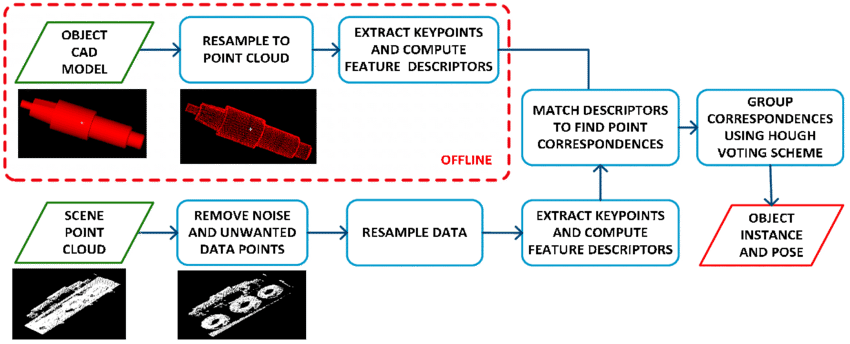
\includegraphics[width=3in]{figures03/pipeline.png}
\caption{General architecture of proposed pose estimation pipeline}%\cite{temp2}}
\label{fig:pipeline}
\end{center}
\end{figure}




\subsection{Filtering a Point cloud}
The point cloud from the output sensory device contains undesired points, those are often noisy and contains outliers that lead to a high computation time and possibly produces a wrong pose estimation of object. Therefore, it is crucial to remove the noise and outliers from the point cloud in order to obtain accurate point clouds that are suitable for further processing. 

In order to identify these suitable point clouds, algorithms for filtering them are already implemented in the Point Cloud Library such as Conditional Removal, Radius/Statistical Outlier Removal, Color Filtering and Passthrough. 
Since there are few widely used techniques already developed for point cloud filtering. Some of them are aimed at reducing the amount of points in order to speed up the computation time. Others are used to discard outliars. In this thesis we exploit a simple and commonly used filtration pipeline which it has been proven to be an effective combination of methods in several works \cite{algFiltering}.

\subsubsection{Filtering a PointCloud using a PassThrough filter}
PassThrough passes points in a cloud based on constraints or threshold for one particular field (X,Y,Z) of the point type. Namely, it removes points where values of selected field are out of range. The filtration pipeline can be seen in the Figure \ref{fig:passthrough}. For more details and working examples the reader you should refer to \cite{pcl}

\begin{figure}[!h]
\begin{center}
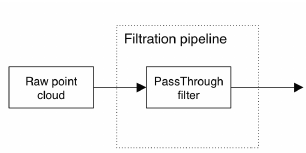
\includegraphics[width=3in]{figures03/passthrough.png}
\caption{Filtration pipeline used in this thesis}%\cite{temp2}}
\label{fig:passthrough}
\end{center}
\end{figure}


\subsection{Preprocessing stage}

After the filtering step, which is only applied to the point cloud represented the scence. The two clouds are downsampled with technique already implemented in the Point Cloud Library, such as Voxelgrid (VG) filter or Approximate Voxelgrid filtering. This step is required for speed up the computation process. 
Since it is a computer vision problem known as Tabletop, it has a dominant plane. Therefore, RANSAC is used to find this dominat plane in the image. 

\subsubsection{Downsampling a PointCloud using a VoxelGrid filter}

Voxel Grid filtering method \cite{algFiltering} creates a 3D Voxel Grid
(3D boxes in 3D space) for each one of the point cloud (model and scene cloud). Then, in each voxel, a point is chosen to approximate all the points that lie on that voxel. Usually, the centroid (an arithmetic mean) of these points or the center (the point in the interior that is equidistant from all points) of this voxel is used as the approximation. The centroid is slower than the center approximation. As a remark, the voxel grid method often drives to geometric information loss. See Figure \ref{fig:voxeldown} to see the result of applying voxel grid. For more information about this filtering, the reader should see \cite{algDownsampling}


\begin{figure}[!h]
\begin{center}
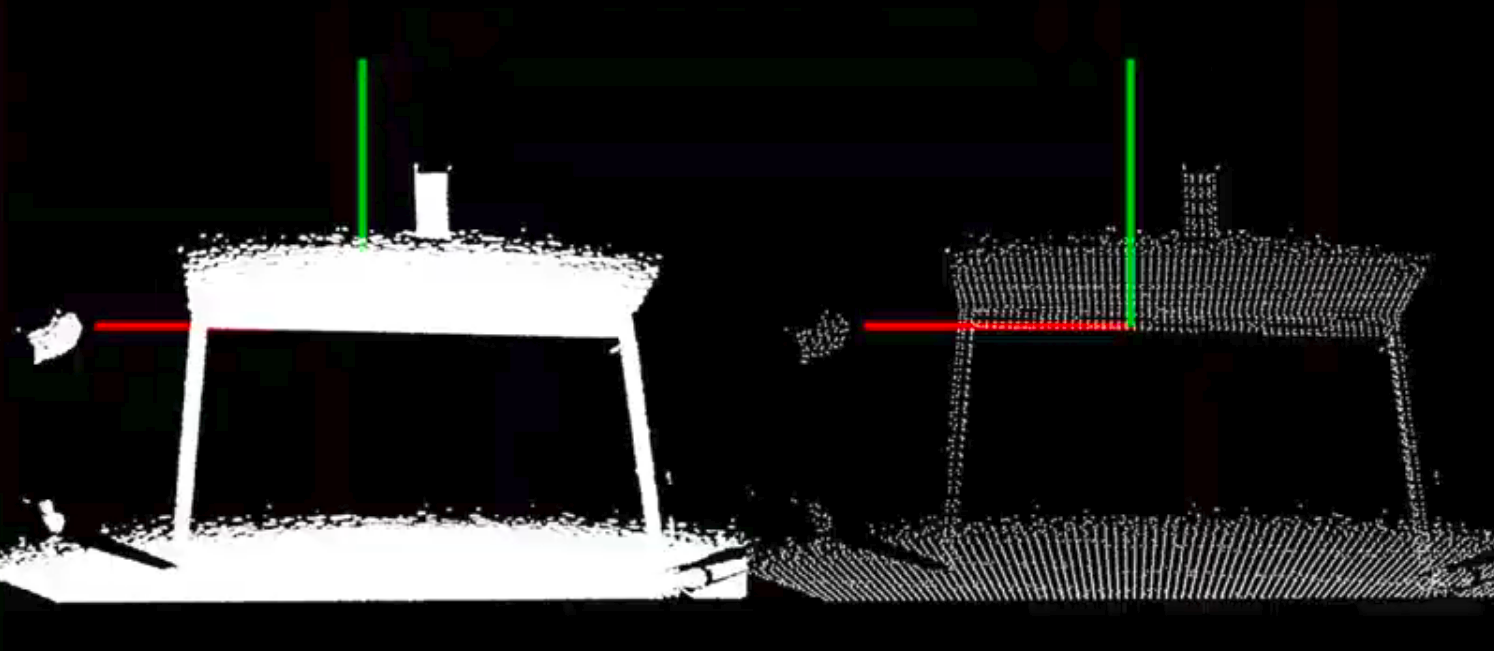
\includegraphics[width=3in]{figures03/voxelcloud1.png}
\caption{Left to Right: Input Image, Output after voxelGrid}%\cite{temp2}}
\label{fig:voxeldown}
\end{center}
\end{figure}


\subsubsection{Plane Segmentation}
Since the point cloud from the scene contains undesirable points such as points that represents a table where the object is kept. A further filtering is needed, such filtering is know as plane segmentation. And it is achievable with the RAMSAC based plane fitting method. RAMSAC method finds the largest set of points that fit to a plane. The plane equation in three dimensional point cloud can be defined as:

\begin{equation}
    ax+by+cz+d=0
\end{equation}
Where the a,b, and c are the parameters of the plane and d is the distance of the plane from the origin.

RAMSAC selects randomly three points from dataset and computes the parameters of the corresponding plane, after that it tries to enlarge the plane according to a given threshold,\cite{algPlane}. The step of segmenting the plane in order to remove it, is required condition for the subsequent use. Where a global registration is applied. 
\\

\begin{algorithm}[H]
\SetAlgoLined
\KwResult{ o (object candidate point cloud) }
\KwData{p (3D point cloud), $\tau$ , MaxIter, IR }
 initialization\;
 \While{$t<MaxIter$ - $InlierRatio>IR$}
 {
 Pick 3 points (A, B, C) at random from p \;
 Fit a plane (ax + by + cz + d = 0) to these 3 points\;
    AB = B - A\;
    AC = C - A\;
    N = AB x AC\;
    N has the values of (a, b, c)\;
    %d = −A^{T} \cdot N\\  
    Find outlier points o (object candidate points)\\
    %f(x)$>$\tau\\
    Here, f (x) is plugging in point x into the plane equation divided by the norm of N to measure residual and $\tau$ is the threshold\\
    Find Inlier Ratio as ratio of number of inlier points to total number of points
}
\caption{RANSAC for plane segmentation \cite{cadPipeline3}}
\end{algorithm}



\subsection{Feature descriptor}

